Looking at the reasonable choices we have derived for our cannonical coordinates, we see we could choose $V,Q.\phi,I$. We know we can say:
\begin{align*}
	m\omega_p^2 &= \frac{e^2 n}{\epsilon_0}
\end{align*}
Describes the motion of an electron in opposition to the overall motions of electrons in a metal. Looking at this frequency, it happens to be extremely large compared to our temperature $\hbar\omega_p \gg k_B T$, for even room temperature. Therefore we should be able to ignore most of our degrees of freedom. If we write our Hamiltonian for the circuit we say:
\begin{align*}
	\mathcal{H} &= \frac{Q^2}{2C} + \frac{\phi^2}{2L}
\end{align*}
Of course we need to add some aharmonicity to our circuit in order to make this a useful qubit. In order to do this we introduce a Josephson junction. We start by considering adding a pair of electrons to a pair of Hydrogen atoms.
Clearly the first electron we add could go to either atom, or a superposition of both atoms. In order to minimize the energy the first electron will go into a state $\frac{\ket{1s}_A + \ket{1S}_B}{\sqrt{2}}$.
The second atom will be put into the same spatial state, but with opposite spin, this overall state is known as the singlet state.
This corresponds to a center of mass state in the singlet state. When we move to a superconducting system, we have all electrons creating a single center of mass state, and therefore all electrons must be in spin pairwise singlet states.

\begin{figure*}[h]
	\centering
	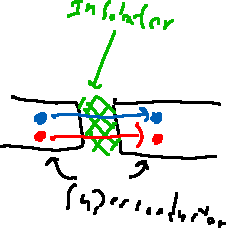
\includegraphics[width=6cm]{12-04-1.png}
	\caption*{A Josephson junction, with electron pairs tunneling across the insolator}
\end{figure*}
A Josephson junction occurs when you take two superconductors and place an insolator between them. This corresponds to the Hamiltonian:
\begin{align*}
	\mathcal{H} &= -\frac{E_J}{2}(\ket{m}\bra{m+1} + \ket{m+1}\bra{m})
\end{align*}
Which describes tunneling of our electron pairs through the insolator (where $m$ is the number of pairs).
We Fourier transform our number states:
\begin{align*}
	\ket{\phi} &= \sum_n e^{in\phi} \ket{n} \\
	\mathcal{H}\ket{\phi} &= -\frac{E_J}{2}\left(\sum_n e^{in\phi}\ket{n-1} + \sum_ne^{in\phi}\ket{n+1}\right) \\
	\mathcal{H}\ket{\phi} &= -\frac{E_J}{2}\left(e^{i\phi}\sum_n e^{in\phi}\ket{n} + e^{-i\phi}\sum_ne^{in\phi}\ket{n}\right) \\
	\mathcal{H}\ket{\phi} &= -E_J\cos\phi\sum_n e^{in\phi}\ket{n} \\
	\mathcal{H}\ket{\phi} &= -E_J\cos\phi\ket{\phi}
\end{align*}
So then our overall Hamiltonian for the LC Joesphson Junction circuit is:
\begin{align*}
	\mathcal{H} &= \frac{Q^2}{2C} + \frac{\phi^2}{2L} - E_J\cos\phi
\end{align*}
This value of $\phi$ additionally can be thought of as the phase between our superconductors. If we think of $Q$ as the momentum then this looks like a single particle in a potential.
In actuallity the only component we need is the Josephson junction, as it has a physical capacitance, and the contribution that our inductor has to the circuit is a $\phi^2$ term that already exists in the $\cos\phi$ terms taylor expansion.

For our superconducting qubit we want to create a circuit including some number of Josephson junctions, and we want it to have a ground state to first excited state transition that is smaller than the first excited state to second excited state transition.
We also want random fluctuations to shift the ground and first excited states by the same amount.

In order to look at measurements on our superconducting qubits we now need to turn to the subject of cavity QED. In this we look at electromagnetic modes in cavities that only support certain wavelengths.
In these optical cavities you can do many different thinks, such as suppressing the spontaneous emission of an atom. You can also cause an atom to exchange energy back and forth with electromagnetic waves in the cavity.
The Hamiltonian for an atom in a cavity can be written:
\begin{align*}
	\mathcal{H} &= \hbar (\omega_0 \unit + g\sigma_x)
\end{align*}
This hamiltonian has shifted energies from the base atoms, instead having energy $E = \hbar(\omega_0 \pm g)$
By putting our qubit in a cavity, we can use the effects of a cavity to shift the energy levels. Additionally the different states of the qubit will modify the transmission of the radiation through the cavity.
Since the difference in transition rates is $~20\%$, vs $~30\%$, distinguishing these states is very difficult.

In order to do two qubit gates, we have two qubits coupled to the same cavity. For this we can write a Hamiltonian:
\begin{align*}
	\mathcal{H}_\text{cavity} &= \frac{\hbar\omega_c}{2}(1 + 2a^\dagger a)
\end{align*}
Here we can then use the same approach we used for Ions in an ion trap to do our two qubit gate.
